\documentclass[english]{beamer}
\usepackage[english]{babel}
\usepackage[utf8]{inputenx}
\usepackage[T1]{fontenc}      % Font encoding
\usepackage{lmodern}          % lmodern font, correctly copyable characters in pdf

\usetheme[
  bullet=circle,                  % Use circles instead of squares for bullets
  titleline=false,                % Show a line below the frame
  alternativetitlepage=true,      % Use the fancy title
  titlepagelogo=logo-sapienza,    % Logo for the first slide
  watermark=watermark-diag,   % Watermark used in every slide
  watermarkheight=20px,           % Desired height of the watermark
  watermarkheightmult=6,          % Watermark image is actually x times bigger
  displayauthoronfooter=true,     % Display author name in the footer
]{Roma}
\watermarkoff
\author{Dario Loi, Davide Marincione, Benjamin Barda}
\title{Mine-RPN}
\subtitle{Or how we were able to recognize pigs et. familia in Minecraft}
\institute{Bachelor's degree in\\ Applied Computer Science and Artificial Intelligence \\ Sapienza, University of Rome}
\date{A. Y. 2021 - 2022}

\begin{document}

\begin{frame}[t,plain]
\titlepage
\end{frame}

\begin{frame}{Behold, data!}
  \begin{figure}[h]
      \centering
      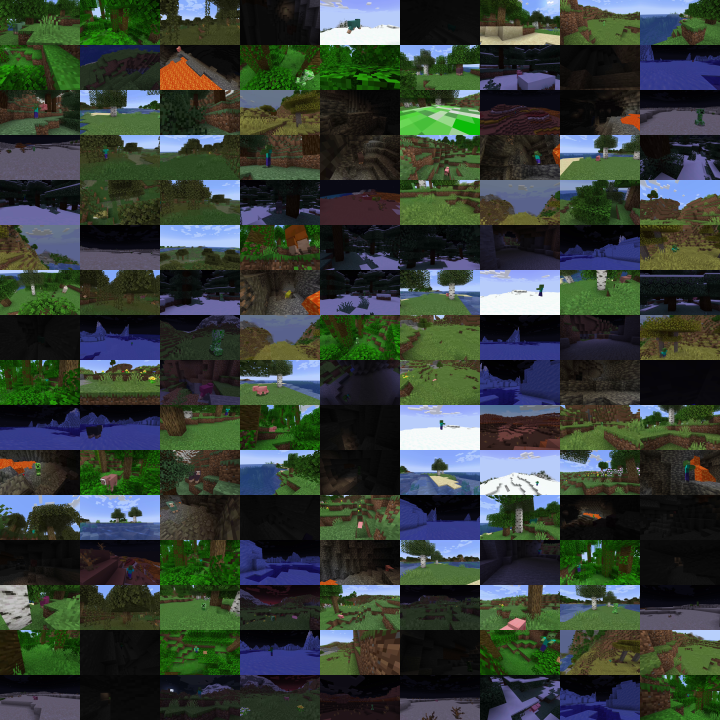
\includegraphics[width=0.5\textwidth]{../images/dtset_repr.png}
      \caption{A representative chunk of our dataset}
  \end{figure}
\end{frame}



\end{document}